\usetikzlibrary{calc}

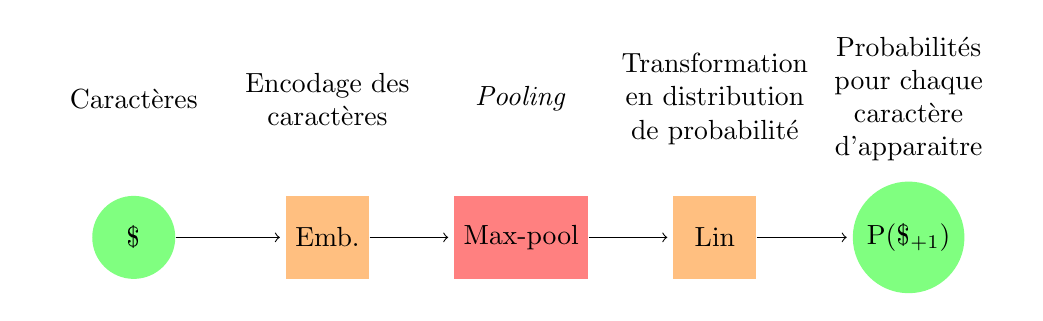
\begin{tikzpicture}[shorten >=2pt,->,draw=black, node distance=7em]
    \tikzstyle{every pin edge}=[<-,shorten <=2pt]
	\tikzstyle{module}=[minimum size=3em, fill=gray!50!]
	\tikzstyle{char}=[module, circle, fill=green!50!]%, label={below:\usebox\mydictbox}]
	\tikzstyle{text label}=[rectangle, text centered, text width=7em, node distance=5em]
	\tikzstyle{nn}=[rectangle, module, fill=orange!50!]
	\tikzstyle{rnn}=[nn, fill=red!50!]

	\node[char] (char) {\$};
	\node[nn, right of=char] (emb) {Emb.};
	\node[rnn, right of=emb] (rnn) {Max-pool};
	%\draw[->] (rnn.north) to [out=90,in=90, looseness=2] ($(rnn.west) + (-0.5,0)$) to [out=-90,in=-90, looseness=2] (rnn.south);
	\node[nn, right of=rnn] (lin) {Lin};
	\node[char, right of=lin] (out) {P(\$$_{+1}$)};
	\draw[->] (char) to (emb);
	\draw[->] (emb) to (rnn);
	\draw[->] (rnn) to (lin);
	\draw[->] (lin) to (out);
	%\node[char] (char) {\$};


    \node[text label, above of=char] (charl) {Caract\`{e}res};
    \node[text label, above of=emb] (embl) {Encodage des caract\`{e}res};
    \node[text label, above of=rnn] (rnnl) {\textit{Pooling}};
    \node[text label, above of=lin] (linl) {Transformation en distribution de probabilit\'{e}};
    \node[text label, above of=out] (outl) {Probabilit\'{e}s pour chaque caract\`{e}re d'apparaitre};
\end{tikzpicture}